\documentclass[final]{article}
\usepackage[english]{babel}
\usepackage{csquotes}
\usepackage{array}
\usepackage[margin=1in]{geometry}
\usepackage{pdfpages}
\usepackage{subcaption}
\usepackage{graphicx}
\usepackage{hyperref}
\usepackage{tablefootnote}
\usepackage{cleveref}[2012/02/15]% v0.18.4; 
\usepackage[table]{xcolor}
\graphicspath{ {./images/} }
  
\usepackage{chngpage}

\usepackage[
backend=biber,
citestyle=ieee,
bibstyle=ieee,
sorting=none,
natbib=true,
maxcitenames=100,
dashed=false,
giveninits=true
]{biblatex}
\renewcommand*{\finentrypunct}{\addperiod\\}% To put white spaces between references
\addbibresource{references.bib}


\usepackage[obeyDraft]{todonotes}
\usepackage[toc,page]{appendix}
\usepackage[nottoc]{tocbibind}
\usepackage[shortlabels]{enumitem}
\usepackage{hhline}
\usepackage{lscape}
\usepackage{tabularray}
\usepackage{comment}


\newcommand{\hreffootnote}[1]{\footnote{\href{#1}{#1}}}
\crefformat{footnote}{#2\footnotemark[#1]#3}
\newcommand{\parenref}[1]{(\ref{#1})}
\newcommand{\cross}[0]{\includegraphics[scale=0.025, draft=false]{cross}}
\newcommand{\checkmark}[0]{\includegraphics[scale=0.025, draft=false]{check}}

\setlength{\arrayrulewidth}{0.3mm}
\setlength{\tabcolsep}{2pt}
\renewcommand{\arraystretch}{1.5}
\newcolumntype{s}{>{\columncolor[HTML]{aabded}} p{1cm}}
\arrayrulecolor[HTML]{fafbfc}

\overfullrule=0pt

% Changes the title of the TOC from "Contents" to "Table of Contents"
\addto\captionsenglish{
    \renewcommand*\contentsname{Table of Contents}
}

\begin{document}
\DeclareFieldFormat{url}{\url{#1}} % To make sure the references page stops rendering the word 'URL'.

% These "TC: ignore comments" are used to prevent sections from counting towards the word count
%TC: ignore
\listoftodos
%TC: endignore

%TC: ignore
\newgeometry{right=1.2in,left=1.2in}
\begin{titlepage}
    \begin{center}
        \vspace*{1cm}
        \huge \textbf{Battle of the Qubits: Metrics for Different Qubit Types and their Future Prospects}
        
        \vspace{0.15cm}
        
        \Large QIST4200

        \vspace{0.2cm}
        
        \normalsize October 2024
        \vspace{1.5cm}

        Ioana-Lisandra Drăgănescu: 5567068, s4122968\\
        Vincent Groen: 5046009, s4552512\\
        Nian Tian Lin: 5053781, s3665453\\
        Tianchen Qu: 5480469, s4569849\\
        Edgar Roussel: 6352561, s4411269\\
        Batuhan Yavuz: 4952901, s4592638\\
        
        \vspace{1.0cm}
        
        \includegraphics[width=\textwidth]{qubit_battle.png}

        \vspace{0.5cm}
        \textbf{Client: } Jan Krzywda\\
    \end{center}
\end{titlepage}
\restoregeometry
%TC: endignore

\pagenumbering{roman}

%TC: ignore
\tableofcontents
%TC: endignore



\clearpage

\pagenumbering{arabic}

\section*{Summary}
This report examines and gives an overall review on six different types of qubits (superconductor, semiconductor spin, neutral atom, trapped-ion, bosonic, and photonic) that are widely discussed today. The report focuses on different metrics for these qubits in the form of a table and discuss their future potentials. This is done specifically under the lens of Fault-Tolerant Quantum Computing (FTQC) which this report considers to be the future direction of quantum computing. This report also provides the reader with reviews in a case-by-case manner for each qubit type. 

\section{Introduction}
With the current knowledge, it is nearly impossible to achieve fault-tolerant quantum computing (FTQC) without proper error correction \cite{roffe2019quantum}, \cite{devitt2013quantum}. Quantum error correction (QEC) aims to recover quantum information that is lost when conducting operations with qubits \cite{roffe2019quantum}. The field of QEC is currently broad: various error correction methods can be used, which can themselves be applied to different qubits, each with its own characteristics \cite{roffe2019quantum}. Therefore, having an overview of the current state-of-the-art QEC, together with suggestions of research directions, can help researchers determine what to focus on. \par

The aim of this report is to present an overview of the state-of-the-art QEC, as well as provide suggestions for the most promising research directions. To achieve this, a literature review was conducted. Perplexity AI \footnote{https://www.perplexity.ai/} was used as a starting point for collecting sources on the topics of interest. Then, the search was extended by examining the sources referenced in the initial papers and by performing Google Scholar \footnote{https://scholar.google.com/} queries with similar keywords. The advantages and disadvantages of six qubit types (superconductor, semiconductor spin, neutral atom, trapped-ion, photonic, and bosonic) were analyzed. This information was then used to spark a discussion about which types are the most promising for QEC. \par

The report is structured as follows. Chapter \ref{section: qec} analyses the potential of six qubit types in the context of QEC. Next, Chapter \ref{section: conclusion} compiles our suggestions and conclusions. \par


% paragraph 1: background
% - background info on the subject
% - problem that needs to be solved
% - importance

% paragraph 2: aim
% - research question/aim
% - methods
% - limitations

% paragraph 3: structure\label{section: introduction}
\clearpage
\section{Suitability of Different Qubit Types for Quantum Error Correction}
\label{section: qec}
In the following section, different qubit types will be compared for their potential to be used in FTQC. For usable QEC, DiVincenzo proposed five basic requirements of an ideal qubit: sufficiently long T1/T2 times (i), fast and reliable gate operations (ii), initialization (iii) and readout (iv), and scalability for large-scale architectures (v) \cite{DIVINCENZO1998419}.  Additionally, the implementation of QEC is partly determined by noise type, working temperature and connectivity. Table \ref{tab:qubit_comparison} contains a comprehensive overview of superconducting, semiconducting, neutral atom and trapped-ion qubits using these metrics. The specifics for each qubit type will be expanded upon in the following subsections.
%Each of these metrics impacts how QEC is implemented. 

%Longer T1 and T2 times, and faster gate speed imply more gate operations before a qubit it loses its quantum state, while higher gate fidelity may reduce control signals. Furthermore, faster initialization and readout, with higher fidelity, will decrease non-circuit related error corrections. Additionally, while lower temperatures mean less decoherence and thermal noise, a higher working temperature gives leeway to simpler cooling systems and better scalability. Finally, noise type and connectivity determine what QEC method is applied. 

\begin{comment}
\begin{figure}
    \centering
    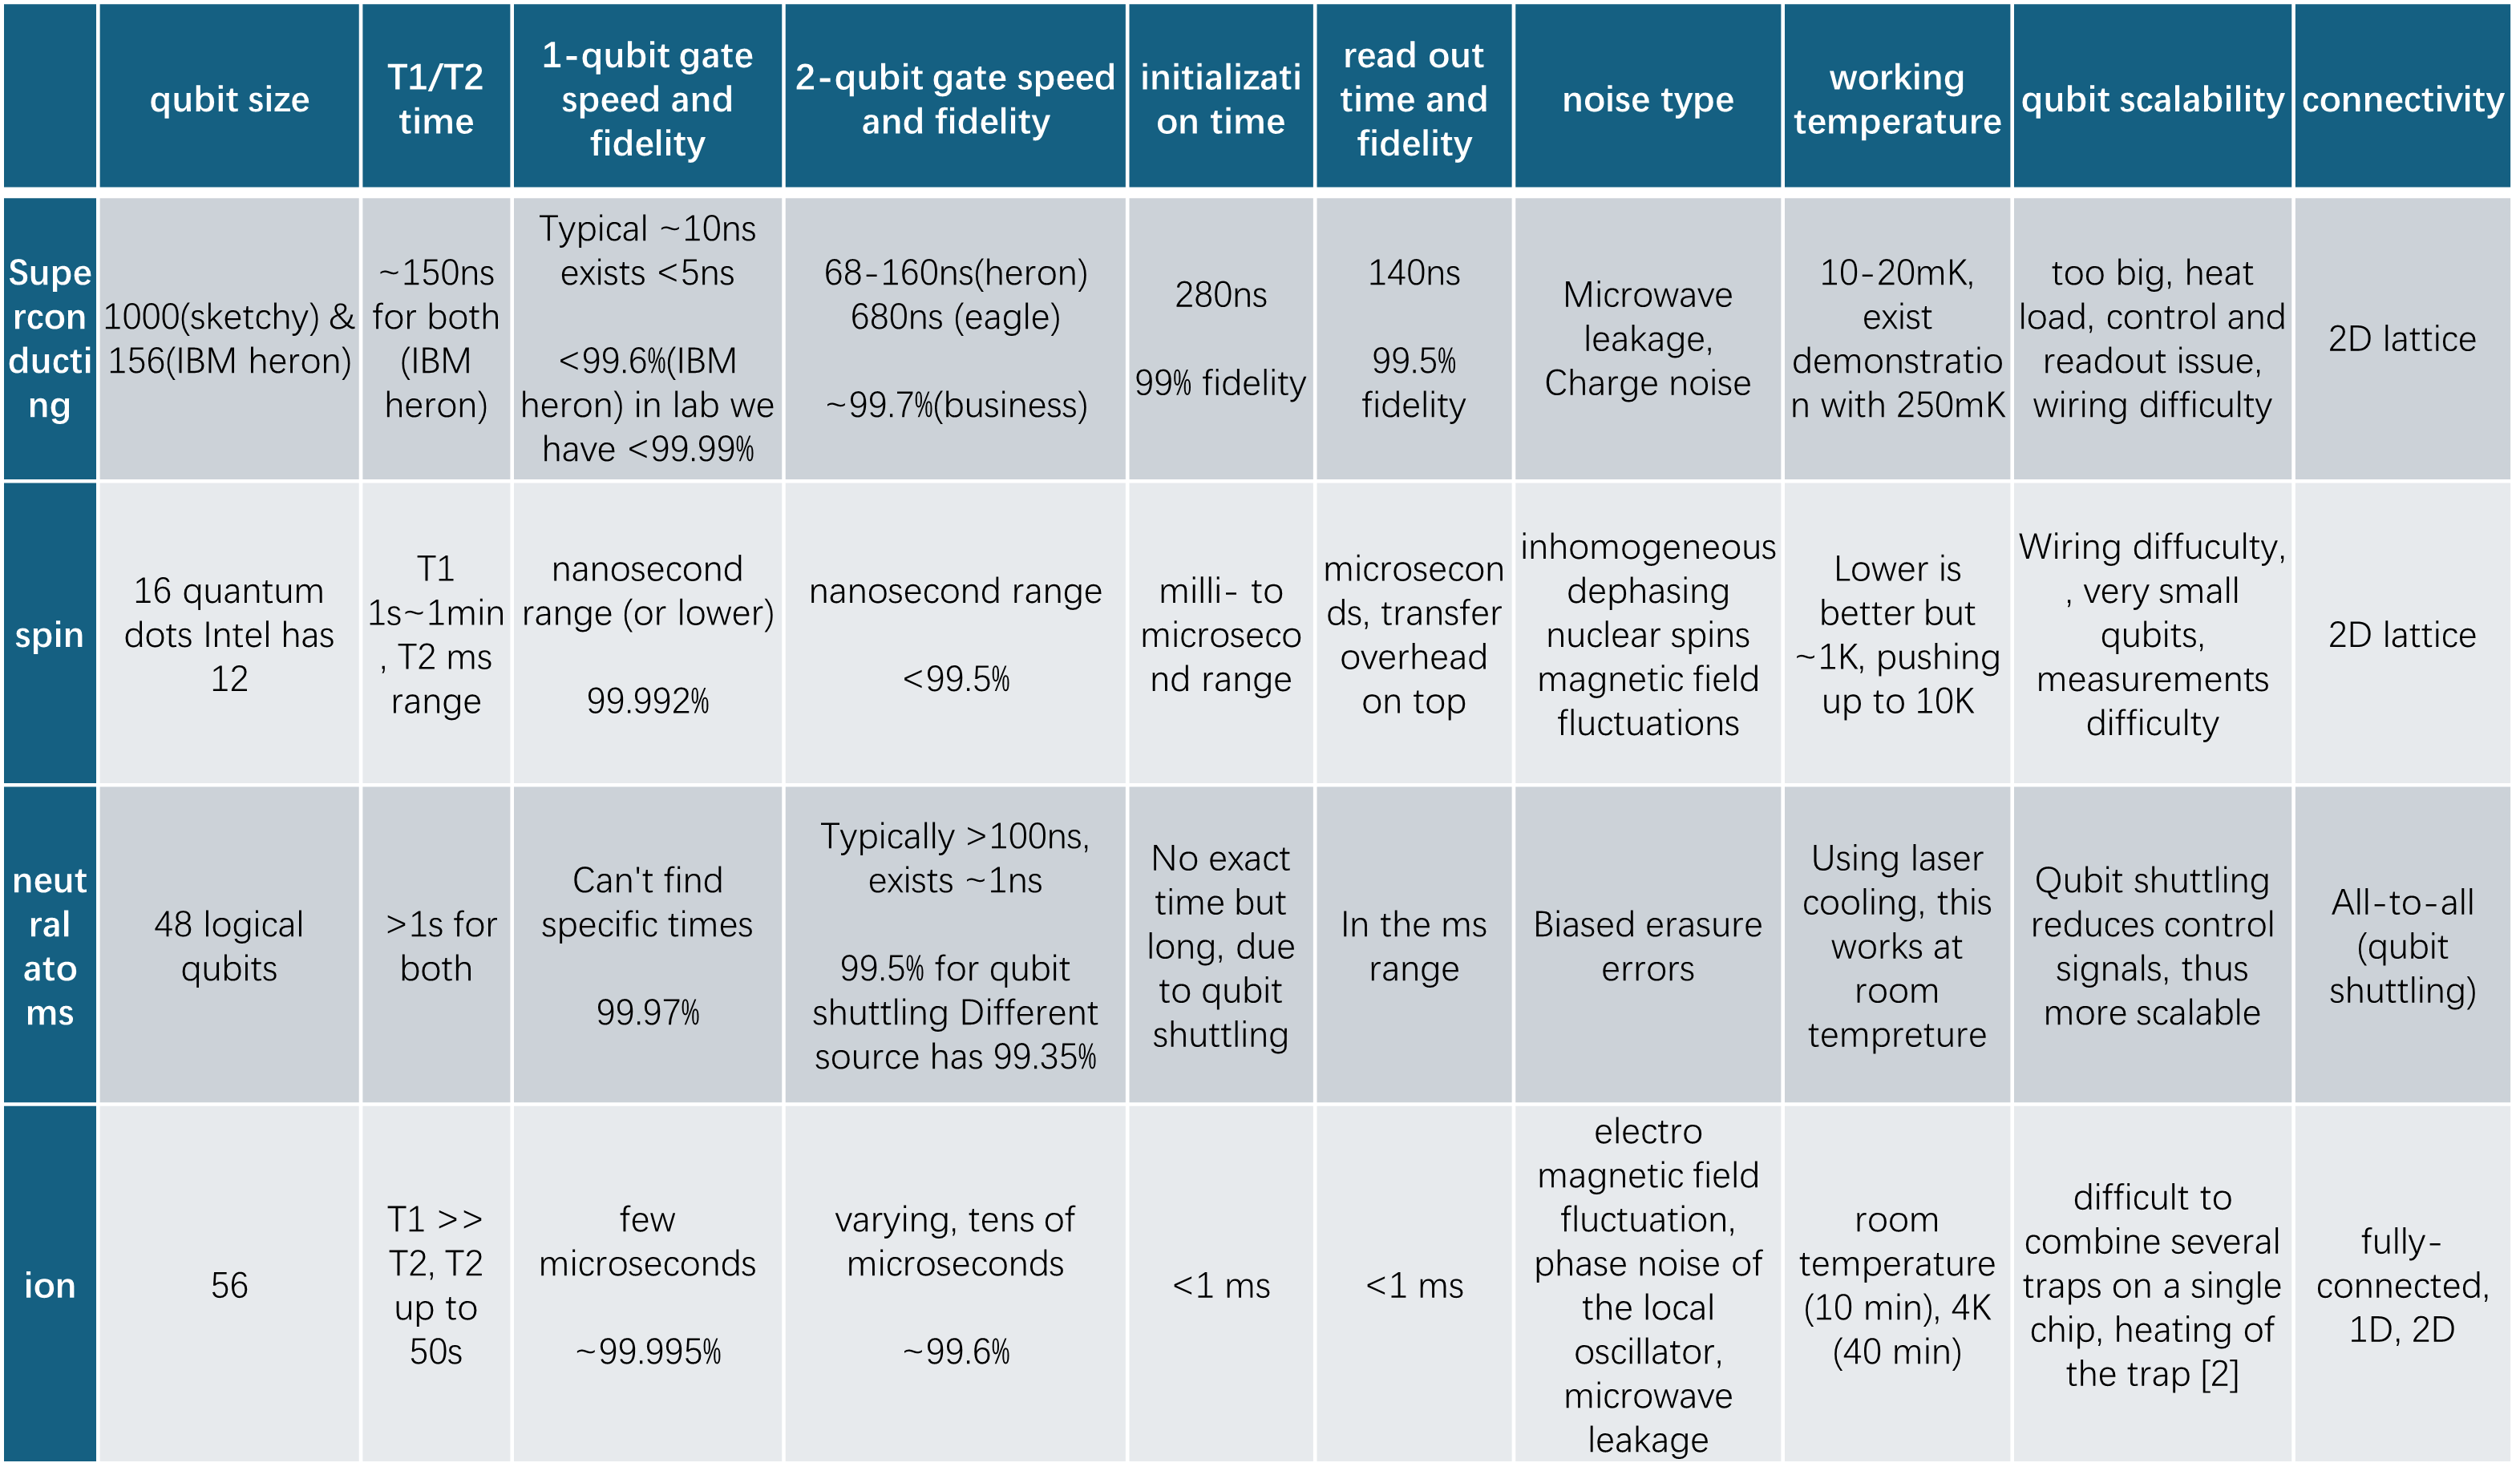
\includegraphics[width=1\linewidth]{images/compare.png}
    \caption{Comparison between different metrics for superconducting, spin, neutral atoms and ion qubits}
    \label{fig:enter-label}
\end{figure}
\end{comment}
% \begin{table}[ht]
% \small
% \centering
% \caption{Stuff}
% \label{tab:1}
%     \begin{tabular}{|p{1cm}|p{1.5cm}|p{1.5cm}|p{1.5cm}|p{1.5cm}|p{1.5cm}|p{1.5cm}|p{1.5cm}|p{1.5cm}|p{1.5cm}|l|} \hline  
%          \rowcolor[HTML]{2f7790}&  \textcolor{white}{Qubit Size}&  T1/T2 time&  1-qubit gate speed \& fidelity&  2-qubit gate speed \& fidelity&  initia-lization time&  readout time\& fidelity&  noise type&  working temperature&  qubit scalability&connectivity \\ \hline  
%          \rowcolor[HTML]{b6bac4} \cellcolor[HTML]{2f7790}super-conduc-ting&  j &  &  &  &  &  &  &  &  & \\ \hline  
%          \rowcolor[HTML]{d9dbe2} \cellcolor[HTML]{2f7790}spin&  &  &  &  &  &  &  &  &  &\\ \hline  
%          \rowcolor[HTML]{b6bac4} \cellcolor[HTML]{2f7790}neutral atom&  &  &  &  &  &  &  &  &  &\\ \hline  
%          \rowcolor[HTML]{d9dbe2} \cellcolor[HTML]{2f7790}ion&  &  &  &  &  &  &  &  &  &\\ \hline 
%     \end{tabular}
    
    
% \end{table}
%TC:ignore
\begin{table}[h]\begin{center}
    \caption{Comparison between different metrics for superconducting, spin, neutral atoms and trapped-ion qubits}
    \label{tab:qubit_comparison}
    \begin{tabular}{|>{\centering\arraybackslash}m{2cm}|>{\centering\arraybackslash}m{3.5cm}|>{\centering\arraybackslash}m{3.5cm}|>{\centering\arraybackslash}m{3.5cm}|>{\centering\arraybackslash}m{3.5cm}|}
         \rowcolor[HTML]{2f7790}&  \textcolor{white}{Superconducting Qubit}& \textcolor{white}{Semiconducting Qubit}&  \textcolor{white}{Neutral Atom Qubit}& \textcolor{white}{Trapped-ion Qubit}\\ \hline
         \rowcolor[HTML]{b6bac4} \cellcolor[HTML]{2f7790} \textcolor{white}{total qubits}&  1121 (IBM Condor)\cite{Afifi-Sabet_2023}, 156 (IBM Heron)\cite{IBMQuantum}& 16 \cite{Borsoi_2023} &  48 logical qubits, 280 physical qubits \cite{Bluvstein2024}& 56 \cite{quantinuum56} \\ \hline
         \rowcolor[HTML]{d9dbe2} \cellcolor[HTML]{2f7790} \textcolor{white}{T1/T2 time}&  $\sim$1.2 ms for both \cite{T1T2}& T1 1 min \cite{Camenzind_2018}, T2\textsuperscript{CPMG} 28 ms \cite{Veldhorst_2014} & T1$\gg$T2, T2 $\sim$40 s \cite{Barnes2022}& T1$\gg$T2, T2 up to 50 s \cite{wang2017single} \\ \hline
         \rowcolor[HTML]{b6bac4} \cellcolor[HTML]{2f7790} \textcolor{white}{1-qubit gate speed \& fidelity}& 4.16 ns\cite{Werninghaus_Egger_Roy_Machnes_Wilhelm_Filipp_2021}, $>$99.99\% \cite{T1T2}& ns range \cite{Stano_2022}, 99.992 \cite{Lawrie_2023}\% & $\mu$s range, 99.97\% \cite{Evered2023}& few $\mu$s, $\sim$99.995\% \cite{bruzewicz2019trapped} \\ \hline
         \rowcolor[HTML]{d9dbe2} \cellcolor[HTML]{2f7790} \textcolor{white}{2-qubit gate speed \& fidelity}& 68 ns (IBM Heron)\cite{IBMQuantum}, $\sim$99.9\%\cite{IQM} & 2 ns \cite{Malinowski_2019}, $\sim$99.81\% \cite{Mills_2022} & typically $>$100 ns \tablefootnote{\label{shuttling} This does not include shuttling time}, 99.5\% \cite{Evered2023}, exists 6.5 ns \cite{Chew2022}& varying, tens of $\mu$s, $\sim$99.6\% \cite{bruzewicz2019trapped} \\ \hline
         \rowcolor[HTML]{b6bac4} \cellcolor[HTML]{2f7790} \textcolor{white}{initialization time}& 180 ns, 99\% fidelity\cite{yoshioka2023activeinitializationexperimentsuperconducting} & ns range, $\sim$99.975\% fidelity \cite{Stano_2022} & $\mu$s to ms range, 99.8\% fidelity \cite{sunami2024scalablenetworkingneutralatomqubits}& $<$1 ms \cite{bruzewicz2019trapped}, 99.93\% fidelity\\ \hline
         \rowcolor[HTML]{d9dbe2} \cellcolor[HTML]{2f7790} \textcolor{white}{readout time}& 140 ns, 99.5\% fidelity\cite{Chen_2023} & $\mu$s range, $\sim$99.975\% fidelity \cite{Stano_2022}& 1 ms \cref{shuttling}, 99.8\% destructive \cite{Bluvstein2024}, 6 ms, 99.6\% non-destructive \cite{radnaev2024universalneutralatomquantumcomputer}& $<$200 $ \mu$s, 99.99\% fidelity \cite{myerson2008high}
or
$<$11 $\mu$s, 99.93\% fidelity \cite{crain2019high}\\ \hline
         \rowcolor[HTML]{b6bac4} \cellcolor[HTML]{2f7790} \textcolor{white}{noise type}&  leakage, charge noise, many others\cite{krantz_quantum_2019}& inhomogeneous dephasing, nuclear spins, magnetic field fluctuations \cite{Sun_2024} & biased erasure errors \cite{Sahay_2023}& EM field fluctuations, phase noise of local oscillator, microwave leakage \cite{wang2021single} \\ \hline
         \rowcolor[HTML]{d9dbe2} \cellcolor[HTML]{2f7790} \textcolor{white}{working temperature}&  250 mK\cite{anferov2024superconductingqubits20ghz} & $\sim$1 K, pushing towards 10 K \cite{Ono_2019} & laser cooling at vacuum room temperature \cite{Wintersperger2023}& room temperature (39 min), 4 K (90 min) \cite{wang2021single} \\ \hline
         \rowcolor[HTML]{b6bac4} \cellcolor[HTML]{2f7790} \textcolor{white}{connectivity}& 2D lattice\cite{IBMQuantum} & 2D lattice & fully connected, 2D, 3D \cite{Bluvstein2024}& fully connected, 1D, 2D \cite{valentini2024demonstration} \\ \hline
         \rowcolor[HTML]{d9dbe2} \cellcolor[HTML]{2f7790} \textcolor{white}{scalability}&  too big, heat load, control and readout wiring issue& wiring difficulty, small qubits, measurement difficulty& reduced control signals, $\gg 10^4$ atoms remains a challenge  \cite{sunami2024scalablenetworkingneutralatomqubits} & difficult to combine several traps on a single chip, heating of the trap \cite{large2024ion} \\ \hline
         
    \end{tabular}
    \end{center}
    
\end{table}
%TC:endignore
\subsection{Discrete Variable Quantum Systems}
These quantum system encode information in finite-dimensional Hilbert spaces, typically encoding information in two-level systems (qubits) or d-level systems (qudits).

\subsubsection{Superconductor Qubits}
Superconducting qubits play a leading role in quantum computing today \cite{acharya2024quantumerrorcorrectionsurface}. With various superconducting quantum processors available, many applications in the Noisy Intermediate-Scale Quantum (NISQ) era can be carried out \cite{IBMQuantum}. Meanwhile, a steady increase in both gate fidelity and qubit number in the past years has been witnessed for superconducting qubits \cite{IBMroadmap}. All these developments also meet the roadmaps from companies such as IBM and Google \cite{IBMroadmap}\cite{Googleroadmap}. Recently, Google has also demonstrated error correction below the surface code threshold for the first time \cite{acharya2024quantumerrorcorrectionsurface}, which sheds light on the path towards the FTQC era.

 Currently, there exist superconducting quantum processors with up to 156 qubits for commercial usage (IBM Heron) \cite{IBMQuantum} and also quantum chips with more than 1000 qubits (IBM Condor). Though high in qubit numbers, the latter one's error rate is five times higher than Heron\cite{Afifi-Sabet_2023}. 
 For the $T_1,T_2^*$ time, around 1.2 ms is achieved via a single fluxonium qubit in lab \cite{T1T2}, together with Clifford gates gate fidelity 99.991\%.
 The single-qubit gate speed can achieve 4.16 ns on a two-qubit platform with gate fidelity 99.76\% via closed-loop optimization for the pulse shape \cite{Werninghaus_Egger_Roy_Machnes_Wilhelm_Filipp_2021}.
 For two-qubit gates, the IBM Heron has 68 ns CZ gate gate with fidelity 99.7\% for a 156 qubits chip.\cite{IBMQuantum} IQM has also demonstrated their CZ gate with 99.9\% fidelity \cite{IQM}.
 For initialization, demonstration in 180 ns with high fidelity has been done for single qubit. This is accomplished by coupling to a quantum-circuit refrigerator through a resonator.
 On the other hand, it took 140 ns for a fidelity 99.5\% two-state readout and a fidelity 96.9\% three-state readout with the help of a feedforward neural network.
 Latest demonstration also showed that the working tempreture can be around 250 mK \cite{anferov2024superconductingqubits20ghz} instead of the usual 10$\sim$20 mK. But this requires higher frequency (up to 24 GHz) and lowloss niobium trilayer junctions.
 
 Fast processing speeds could be a key feature in the FTQC era. Compared to the NISQ era, coherence time for a fault tolerant qubit is not as important since the average gate error is lowered to $\sim10^{-9}$. At the same time, QEC requires a large number of gates, initialization and measurements \cite{Fowler_2012} and fast gate speed is important here. Superconducting qubits are also easy to parallelize operations by using techniques such as Superconducting Quantum Interference Device (SQUID) loops to tune resonant frequencies \cite{krantz_quantum_2019}. The 2D lattice structure for the superconducting qubits also fits many prominent error correction codes such as the surface code as it emphasizes nearest neighbour interaction and local errors \cite{Fowler_2012}. 

However, superconducting qubits also have many drawbacks. Current superconducting qubits and transmission lines are huge compared to other qubits such as spin qubits. A million superconducting qubits on a flat 2D lattice can be square meters large, which could raise problems for clock synchronization since they are running at 4-8 GHz. Heating is a problem due to the low working temperature of superconducting qubits. At 10 mK, cooling power becomes a bottleneck for the number of control and measurement lines to connect to the processor \cite{krantz_quantum_2019}.

% Superconducting qubits do not seem to have many bottlenecks in the near term. However, there still remain obstacles towards the goal of a million physical qubits or 1000 logical qubits. The size of the superconducting circuit and its transmission lines is a persisting issue. Growing qubit number would also require larger and better fridges. 
% Due to the fast gate speed, FPGA could potentially be a big helper for superconducting qubits: On the one hand, it can decrease the classical processing time for the error correction decoder. On the other hand, controlling on the same level as the quantum processor can greatly reduce the control and measurement lines for the chip and lower the cooling power requirement.

\subsubsection{Semiconductor Spin Qubits}

Spin qubits based in a semiconducting medium are, in the long run, among the most promising types of qubits. This is in part due to their inherent compatibility with existing semiconductor manufacturing methods \cite{Zwerver_2022}. Aside from that, spin qubits have been shown to reach a fidelity over the surface code threshold, setting them up as a potential candidate for FTQC \cite{Xue_2022}.

The current state-of-the-art in semiconductor spin qubits promises several advantages over other qubit types. In addition to the previously mentioned fabrication methods, spin qubits are inherently small in size (100 nm), which is an important advantage in scaling of the quantum systems \cite{Neyens_2024}.
Other advantages of this qubit type include the existence of three-qubit (toffoli) gates \cite{Stano_2022} and the possibility to use spin qubits in hot environments, up to 10 K \cite{Ono_2019}.
Importantly for QEC, spin qubits have fast one- and two-qubit gate operations with high fidelity.

The biggest system as of yet can contain and address 16 physical qubits \cite{Borsoi_2023}, however there are still obstacles in the way of scaling semiconducting spin qubits to larger fault-tolerant systems. The most important of these scaling issues has to do with the measurement of qubits. For QEC, it is important that multiple qubits can quickly be measured and initialized. It is impossible to measure every individual qubit simultaneously for spin qubits in larger systems, such as the one by Borsoi et al \cite{Borsoi_2023}. This results in an additional time delay to move a qubit to a sensor.

Furthermore, it is important to discuss several experimental values found in Table \ref{tab:qubit_comparison}.
The T\textsubscript{2}\textsuperscript{CPMG} time has been shown reach periods up to 0.56 seconds in an experiment by Muhonen et al \cite{Muhonen_2014}. In this experiment, a P-donor is used to achieve these long coherence times which is better suited for quantum memory than quantum computing. For this reason, this result was omitted from the table, instead opting for the 28 ms timescale.
It is also important to note that in the setup for the experiment of the 2-qubit gate fidelity by Mills et al \cite{Mills_2022}, a two qubit chip was used. The implication of this setup is that it is not known what the effects of cross-talk would be if this method was scaled up.

Future developments aim to overcome, or work around, some of the previously mentioned obstacles. Progress in hardware and manufacturing methods will result in an increase of the fidelity of operations and coherence times \cite{Stano_2022}. Furthermore, techniques involving qubit shuttling (\cite{Knne_2024}) increase the connectivity of these systems to allow for new QEC implementations.

\subsubsection{Neutral Atom Qubits}

Neutral atom qubits have seen a steadily increasing interest as a promising candidate in the search for scalable FTQC. The fact that neutral atoms are identical qubits, have relatively long coherence times of $\sim$40 s \cite{Barnes2022}, and do not require complex circuitry and wiring compared to other qubit types \cite{ball2024} makes them interesting to investigate. A main feature of this type of qubit is the ability to dynamically reconfigure a qubit array (i.e. shuttling) in a zoned architecture, enabling an all-to-all connectivity between qubits \cite{Bluvstein2024}, \cite{Bluvstein2022}. This array of neutral atoms is laser-cooled and can be freely manipulated using optical tweezers while preserving the coherence and entanglement of the qubits without fidelity cost \cite{Bluvstein2024}, \cite{Wintersperger2023}.

Historically, an important aspect holding neutral atoms back had been the low two-qubit gate fidelity. However, new developments in laser technology have increased the fidelity to 99.5\% \cite{Evered2023}. Combining this higher fidelity with the zoned approach and qubit shuttling has shown significant results, namely the successful execution of an error-corrected quantum processor with 48 logical qubits \cite{Bluvstein2024}, which is the highest number to date \cite{Swayne2023}. The zoned approach can be scaled to $\sim$10,000 atoms by using stronger lasers and it offers constant-space-overhead to QEC, with possible implementations being high-rate quantum concatenated codes and low-density parity (LDPC) codes \cite{sunami2024scalablenetworkingneutralatomqubits}. Nevertheless, scaling beyond this might require further advancements in optical control \cite{Bluvstein2024}, \cite{sunami2024scalablenetworkingneutralatomqubits}.

Some challenges still remain in the slow initialization, gate operation and readout times, which are limited by the physical movement of the qubits. An improvement of these times was demonstrated by introducing an architecture where the qubits are stationary and  a laser is moved around to individually address the qubits using advanced optical control techniques. The gate operation and readout is then limited by optical switching with entangling gate fidelity of 99.35\% \cite{radnaev2024universalneutralatomquantumcomputer}. 
While this technique is faster than qubit shuttling, the ability for all-to-all connectivity is lost in return. Therefore, a potential middle ground might be a hybrid implementation of both optical addressing and qubit shuttling.
Additionally, a newly developed non-destructive readout method also enables the possibility for  mid-circuit readout and error correction \cite{radnaev2024universalneutralatomquantumcomputer}. This reduces the amount of non-circuit operations, such as atom arrangement and loading, leading to faster overall operations.


\subsubsection{Trapped-Ion Qubits}
Trapped-Ion qubits offer a significant number of advantages over other types of qubits, and are thus considered a very promising approach to achieving FTQC \cite{schafer2018fast}, \cite{bruzewicz2019trapped}. To begin with, one of their main assets is their long coherence time. For example, a coherence time of approximately 5500 s (more than 90 min) has been observed for the $^{171}Yb^{+}$ ion qubit \cite{wang2021single}. Moreover, an even bigger advantage of trapped-ion qubits is the fact that they maintain a long coherence time even at room temperature. To detail, a coherence time of 39 min has been achieved at room temperature using ionized donors in $^{28}Si$ \cite{saeedi2013room}. Lastly, trapped-ion qubits allow for high gate fidelities - $99.993-99.999\%$ for single-qubit gates, and $99.3-99.9\%$ for two-qubit gates \cite{bruzewicz2019trapped}. \par

On the other hand, trapped-ion qubits suffer from a number of downsides. Possibly the most relevant disadvantage of using this type of qubits is their gate speed. As it can be observed in Table \ref{tab:qubit_comparison}, the gate speed of trapped-ion qubit systems is several orders of magnitude lower than that of other qubit systems. More precisely, for other types of qubits, it is in the $ns$ range, while it is in the $\mu$s range for trapped-ion qubits \cite{bruzewicz2019trapped}. Additionally, this qubit type suffers from slow advances in scalability, mainly due to difficulties in controlling the individual ions \cite{bruzewicz2019trapped}.  \par

Both the upsides and downsides of trapped-ion qubits reflect in their implementation of QEC. To begin with, the high gate fidelity of trapped-ion qubits allows for the implementation of surface codes \cite{bruzewicz2019trapped}, which are a popular QEC method that manages to correct both bit flips and phase flips \cite{fowler2012surface}. However, their low gate speed (see Table \ref{tab:qubit_comparison}) might make the use of surface codes in larger trapped-ion networks less feasible. As such, other QEC methods have been experimented with since. For instance, dissipation could be used to stabilize qubits \cite{reiter2017dissipative}. Alternatively, shuttling-based or hiding-based QEC schemes could be used \cite{bermudez2017assessing}. \par



% paragraph 3 = qec
% - sufficient gate fidelities -> surface codes work \cite{bruzewicz2019trapped} \cite{fowler2012surface}
% - slow speed - maybe might slow surface codes down - reference table
% - some other codes besides surface codes have been used: dissipative \cite{reiter2017dissipative}, shuttling, hiding \cite{bermudez2017assessing}





% paragraph 1 = upsides: 100-150 words
% - coherence time \cite{wang2021single} - 5500s 171-Yb+
% - room temperature \cite{saeedi2013room} - 39 min at room temp
% - gate fidelities - \cite{bruzewicz2019trapped} - table

% paragraph 2 = downsides: 100-150 words
% - slow gate speed
% - qec not being that happy with it?? - ask jan about it

% paragraph 3 = interaction with fpga
% - tbd after fpga research

\subsection{Continuous Variable Quantum Systems}
These quantum systems encode information in infinite-dimensional Hilbert spaces, encoding information in continuous degrees of freedom such as the quadratures of electromagnetic fields, using quantum harmonic oscillators. These are better known as qumodes \cite{noauthor_introduction_nodate}, which do not share the same characteristics as other qubits. Due to these differing characteristics, they show great potential as a candidate for scalable FTQC and QEC. 


\subsubsection{Bosonic Qubits}
Bosonic qubits are a promising approach to quantum computing, often implemented in superconducting or trapped-ion systems. They have general high fidelity ($\sim$97\%) and increased error correction performance ($\sim$95-98\%) \cite{chatterjee-2023}. Bosonic qubits come in 4 main types: cat, Gottesman-Kitaev-Preskill (GKP), dual-rail, and binomial qubits. Dual-rail and binomial qubits are promising \cite{levine-2024}, \cite{michael-2016}, but dual-rails are still mainly experimental, and binomial qubits are extremely hard to implement and scale. Therefore, they will not be mentioned anymore in this section.


Cat qubits are designed to aim for beyond the NISQ era, and are rapidly being developed by different actors, such as Amazon \cite{chamberland-2022} and Alice \& Bob \cite{alice-bob-2024}. They exhibit exponential decrease in bit-flip errors, leading to coherence times over 10 s \cite{reglade-2024}, 100 s (without quantum control) \cite{berdou-2023} and even possibly exceeding 7 min \cite{alice-and-bob-2024} in different conditions. Cat qubits also promise for low overhead with LDPC codes and a universal set of gates \cite{ruiz-2024}, combined to passive error correction due to their architecture. One of the trade-offs for their inherent bit-flip error protection is a linear increase in phase-flip errors \cite{quera}, requiring other error correction methods. Additionally, maintaining their superposition of states against decoherence requires complex techniques \cite{tucker-2024}, sometimes hard to implement. Cat qubits are also currently mainly implemented on superconducting architecture, requiring extremely low temperatures to operate (around 10 mK), hence enhancing their implementation complexity.

GKP codes originated in 2001 from a paper suggesting encoding a qubit in an oscillator \cite{gottesman-2001}. They are currently being developed by Nord Quantique \cite{nord-UANTIQUE}, the University of Tokyo \cite{konno-2024}, AWS \cite{noh-2022}, and others. They have an inherent protection against both bit-flip and phase-flip errors and require a low overhead for QEC \cite{noh-2022}. GKP codes also drastically reduce hardware requirements for creating a logical qubit, and have very recently been described as the most promising type of bosonic qubit, outperforming other bosonic codes \cite{lemonde-2024}. However, the scaling and implementation complexity of GKP codes are quite a challenge \cite{grimsmo-2021}, adding on to that the need for additional error correction despite their intrinsic error correction capabilities \cite{noh-2022}. Lastly, when one error occurs, GKP codes can efficiently correct for it in a small amount of time. Yet, if in that timespan, another error occurs, the qubit's logical state progressively deteriorates \cite{nord-quantique}.


\subsubsection{Photonic Qubits}

%Photonic qubits are an upcoming and one-of-a-kind approach to quantum computing. Since these qubits implement photons, which are always active, they perform and encode information in the infinite-dimensional Hilbert space of quantum harmonic oscillators, better known as qumodes \cite{noauthor_introduction_nodate}. These photonic 'qumodes' do not share the same characteristics as other qubits. Due to these deviating characteristics, they show great potential as a candidate for scalable and FTQC and QEC. 

Photonic qubits are a specific type of bosonic qubits, encoding information similarly but using photons as information carriers. They therefore do not require using superconducting or other systems.

The current state-of-the-art photonic qumodes are mostly based on theoretical papers that promise great potential, but some experimental papers also show and prove these advantages. 
Photonic qumodes are mainly interesting due to their extremely long coherence values \cite{yan_silicon_2021} and have good scalability, which supports quantum communication and error correction. Since photons are active at room temperature and move at the speed of light, they show high potential for fast and accurate quantum error correction \cite{nourbakhsh_quantum_2022}. Another potential upside to photonics would be that the logical gate speed could potentially be at least 25 times faster than that of superconducting qubits \cite{tezrudolph_what_2023}. 

However, there are two main issues in the current research on photonics. The first one would be due to photon loss, photons can be lost during transmission or manipulation, which can lead to errors in quantum information processing \cite{noauthor_photonic_nodate}. The second problem would be that photons can not stop moving and can not interact with each other, implying that creating a two-qubit gate is difficult to achieve. However, certain methods like LDPC codes \cite{djordjevic_photonic_2009} and Linear Optics Quantum Computing (LOQC) \cite{noauthor_photonic_nodate} are being developed and researched to overcome these problems. 


\begin{comment}
https://www.nature.com/articles/s41586-021-03290-z 
Preserve the qubit information with a fidelity of 96.2 ± 0.3 
We achieve a nondestructive detection efficiency upon qubit survival of 79 ± 3 percent and a photon survival probability of 31 ± 1 percent.
This is used to distinguish the two atomic states |0a⟩ and |1a⟩ with a fidelity of (98.2 ± 0.2) percent at a photon-number threshold of one.

https://outshift.cisco.com/blog/how-powerful-are-photonic-quantum-processors
we present the minimum optical properties required to achieve a QV (quantum Volume = how big the system can get before overwhelmed by too much noise) of 2$^10$, which is a typical value reported for common quantum computing platforms such as superconducting qubits or trapped ions. 

Our findings indicate that photonic hardware would require improvements to reduce losses to approximately 10percent (or 0.5 dB) and a squeezing rate of 18 dB for coherent-pulse qubits to achieve a QV of 2$^10$. To put numbers in perspective, the record squeezing rate ever reported in optics labs around the world is 15 dB. Also, most photon loss events occur at the waveguide interface when the signal enters the chip and is measured at the detector. A typical value of loss rate at the interface is 20 percent (or 1 dB).


https://journals-aps-org.tudelft.idm.oclc.org/prxquantum/pdf/10.1103/PRXQuantum.4.030336
In this work, we report a single-photon qubit encoded in a novel superconducting cavity with a coherence time of 34 ms, representing an order of magnitude improvement compared to previous demonstrations. We use this long-lived quantum memory to store a Schrödinger cat state with a record size of 1024 photons, indicating the cavity’s potential for bosonic quantum error correction.

Our experimental results show a single-photon relaxation time of Tc1 = 25.6 ± 0.2 ms and
a coherence time of Tc2 = 34 ± 1 ms

\end{comment}

\section{Discussion and Conclusion}
\label{section: conclusion}

% Discuss
%   Results
%   Limitations

% Conclusion
%   No free lunch
%   

The purpose of this report was to present an overview of the state-of-the-art for various qubit types. To this end, six qubit types were discussed according to a set of metrics. For each qubit, this report compiled the most optimistic results of recent studies and highlighted the obstacles that need to be overcome in the near future to enable FTQC.

% Results
When looking at the metrics compiled in this report, all qubit types would be feasible for FTQC. While the bosonic and photonic qubits are still mostly theoretical models, quantum computing has been realized for the other four qubits, superconducting, semiconducting, neutral atom, and trapped-ion.
These latter qubits have each, in individual experiments, been shown to be well on their way to the FTQC-era.

% Limitations
This statement, however, also highlights the main limitation of this report. Because only the most optimistic values were considered, the resulting overview is also optimistically biased in favor of these qubit types. It is therefore important to reiterate that most results mentioned in this report were obtained in isolated experiments, where the conditions would have been perfect for each specific case.
This could imply that the setup that allowed for one result to be obtained would hinder another experiment or even make it completely infeasible.

When observing the results of this report, it is clear to see that there is no single best qubit type as of yet. Some qubits may be more developed than others, but each qubit has its own set of advantages and disadvantages.
Choosing a relevant qubit depends on the use-case, in general the superconducting qubit is a relatively mature technology, semiconducting qubits can use existing manufacturing infrastructure for fast scaling, neutral atom and trapped-ion qubits are very stable, and photonic qubits appear ideal for a quantum internet.

Similar to the "no free lunch theorem" for optimization algorithms proposed by Wolpert and Macready in \cite{Wolpert_1997}, the elevated performance of a qubit in one area is usually offset by the performance over another area. Therefore, it is currently impossible to assign one qubit as the best.


%TC:ignore
\clearpage
\printbibliography[heading = bibintoc, title = References]

\clearpage
\appendixpage
\appendix

\section{Work Distribution}\label{section: distribution}
The work has been distributed as follows:
\begin{itemize}  
    \item 3D picture: Edgar Roussel
    \item summary: Tianchen Qu
    \item introduction: Ioana-Lisandra Draganescu;
    \item introduction to Chapter \ref{section: qec}: Timmy Lin;
    \item semiconductor spin qubits: Vincent Groen;
    \item superconductor qubits: Tianchen Qu;
    \item trapped-ion qubits: Ioana-Lisandra Draganescu;
    \item neutral atom qubits: Timmy Lin;
    \item photonic qubits: Batuhan Yavuz;
    \item bosonic qubits: Edgar Roussel;
    \item conclusion: Vincent Groen.
\end{itemize}
%TC:endignore
\end{document}